\newif\ifglobal

%%%%%%%%%%%%%%%%%%%%%%%
%%% Compile to view %%%
%%%%%%%%%%%%%%%%%%%%%%%

%%%%%%%%%%%%%%%%%%%%%%%%%%%%%%%%%%%%%%%%%%%%%%%%%%%
%%% Readme:                                     %%%
%%% https://www.overleaf.com/read/bwdjvfjksvjy/ %%%
%%%%%%%%%%%%%%%%%%%%%%%%%%%%%%%%%%%%%%%%%%%%%%%%%%%

% >>> M?: marks a module setting number or important notice

% >>> M4: Set {./relative-path} to external files for this module <<<
\def \modulefiles {./07-SYSMEM}
% To add an external file, use:
% (Replace '---' with actual filename)
% '\input{\modulefiles/tables/---.tex}' for tables
% '\includegraphics{\modulefiles/figures/---}' for figures
% '\subfile{\modulefiles/---}' for register files


% >>> M1: This module is in global project? <<<
% 'YES' - uncomment; 'NO' - comment out
\globaltrue

\ifglobal
    \documentclass[main\_\_EN.tex]{subfiles}
   
\else
    \documentclass[openany, 10pt]{book}

    % >>> M2: In ./00-shared/preamble-trm-module, also find
    %         settings for visibility of todo notes, watermark <<<
    \usepackage{preamble-trm-module}

    % >>> M3: Temporary labels in English,
    %         you can add your own labels there <<<
    \myexternaldocument{./00-shared/temp-labels-en}

\fi %\ifglobal


\setcounter{secnumdepth}{4}


% >>> M5: If this module needs any updates in
% './00-shared/preamble-trm-module.sty'
% (include additional package, etc.), contact your module PM
% or create the file './00-shared/changelog.tex' make the
% necessary updates yourself and document them in this file <<<


\begin{document}


% Sets language into which pre-defined bits of text are translated
\selectlanguage{english}

% Do not delete this block
\ifglobal
% Add the following front matter if
% this module is outside of global project
\else
    \InputIfFileExists{readme}{}{}
    {\let\clearpage\relax \listoftodos}
    \tableofcontents
    %\listoftables
    %\listoffigures
\fi


%%%%%%%%%%%%%%%%%%%%%%%%%
%%% TRM Module Begins %%%
%%%%%%%%%%%%%%%%%%%%%%%%%

\hypertarget{sysmem}{}
\chapter{System and Memory} 
\label{mod:sysmem}

\section{Overview}

The \chipname{} is an ultra-low-power and highly-integrated system with a 32-bit RISC-V single-core processor with a four-stage pipeline that operates at up to 160 MHz. All internal memory, external memory, and peripherals are located on the CPU buses.

\section{Features}

\begin{itemize}
    \item {\bfseries Address Space}
        \begin{itemize}
    	    \item 792 KB of internal memory address space accessed from the instruction bus 
    	    
    	    
    	    \item 552 KB of internal memory address space accessed from the data bus 
    	    
    	    
    	    \item 836 KB of peripheral address space
    	    \item 8 MB of external memory virtual address space accessed from the instruction bus
    	    \item 8 MB of external memory virtual address space accessed from the data bus
    	    \item 384 KB of internal DMA address space
        \end{itemize}
    \item {\bfseries Internal Memory}
        \begin{itemize}
            \item 384 KB of Internal ROM
	        \item 400 KB of Internal SRAM
	        \item 8 KB of RTC Memory
	    \end{itemize}
    \item {\bfseries External Memory}
        \begin{itemize}
            \item Supports up to 16 MB external flash
	    \end{itemize}
    \item {\bfseries Peripheral Space}
        \begin{itemize}
           \item 35 modules/peripherals in total
        \end{itemize}
    \item {\bfseries GDMA}
        \begin{itemize}
            \item 7 GDMA-supported modules/peripherals
        \end{itemize}
\end{itemize}

Figure \ref{fig:sysmem-address-mapping-structure} illustrates the system structure and address mapping.

\begin{figure}[H]
    \centering
    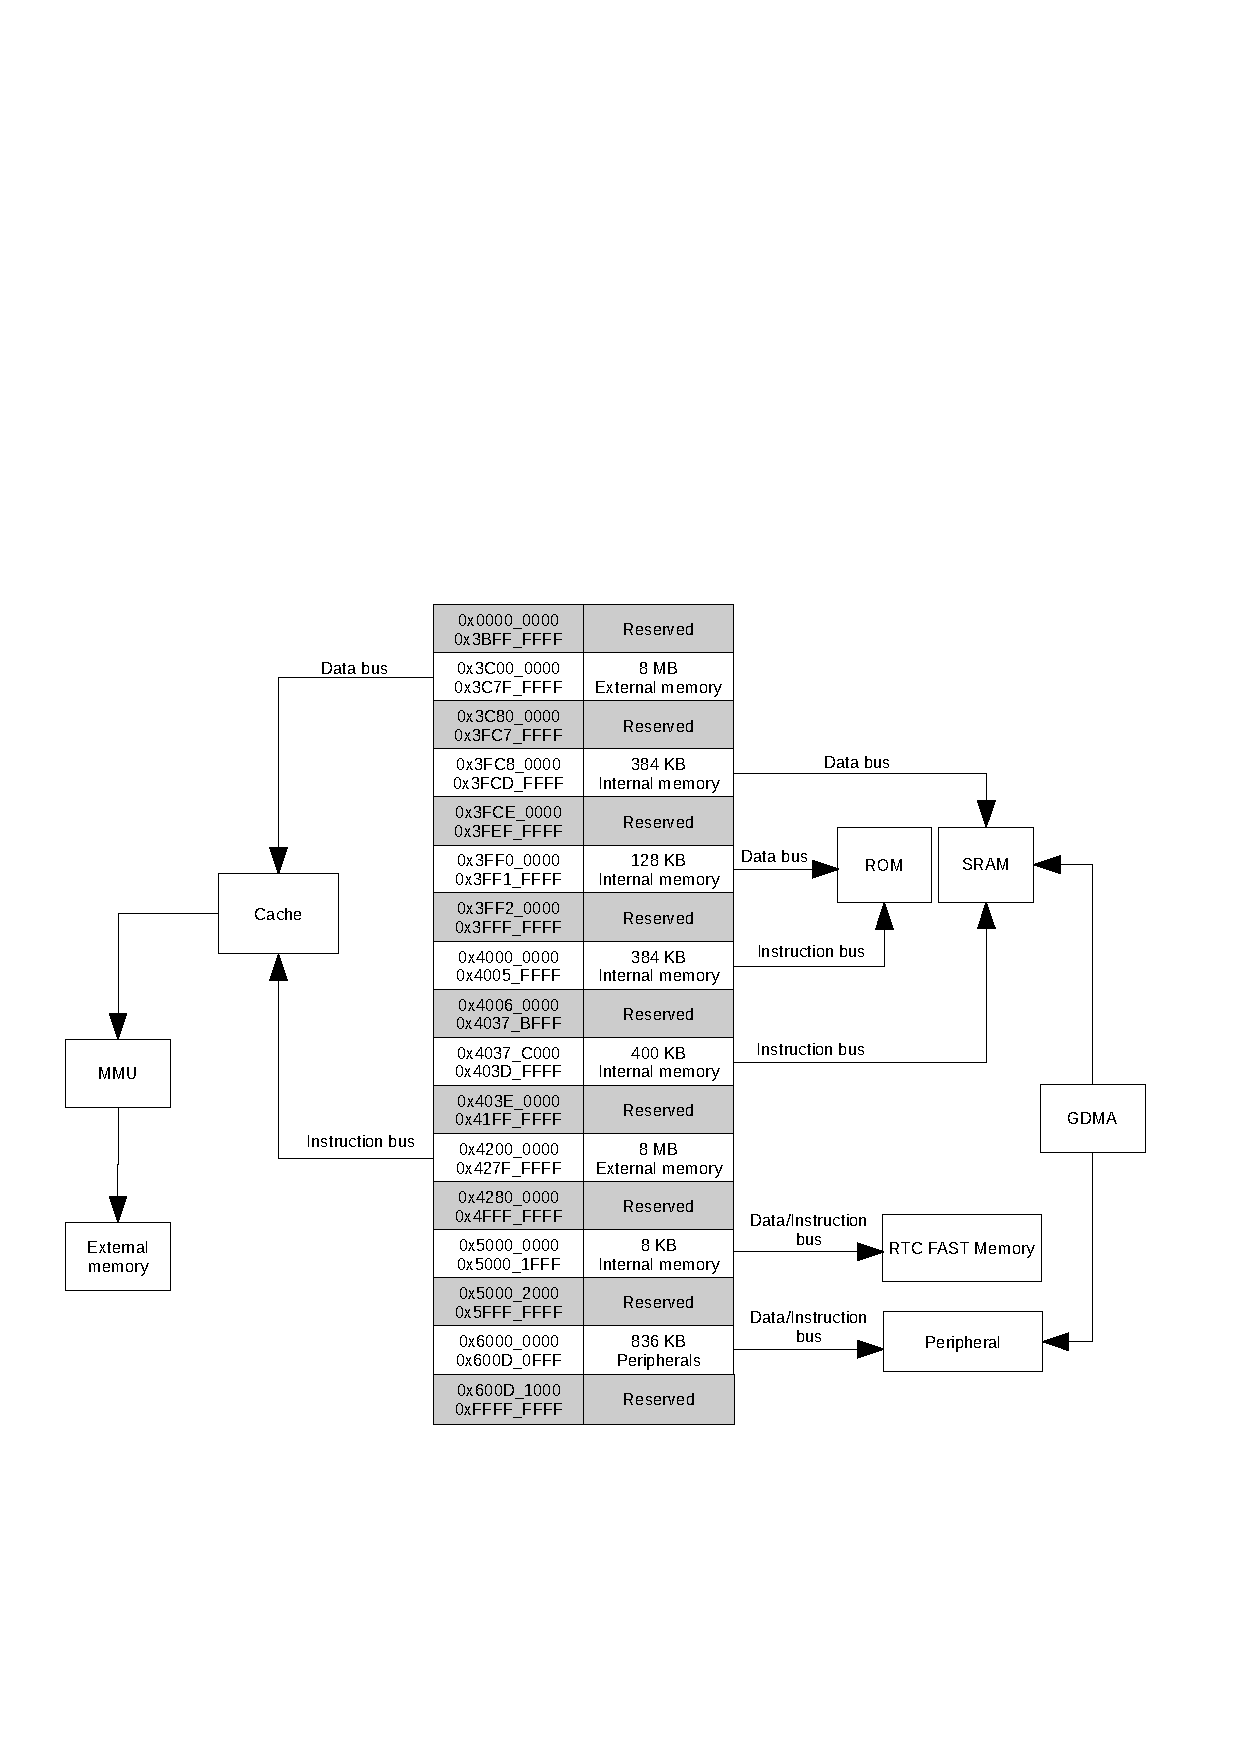
\includegraphics[width=1.0\textwidth]{./07-SYSMEM/figures/07-SYSMEM-addr-mapping.pdf}
    \caption{System Structure and Address Mapping}
    \label{fig:sysmem-address-mapping-structure}
\end{figure}

\begin{tiplisting}
\vspace{-2em}
\begin{itemize}
    \item The address space with gray background is not available to users.
    \item The range of addresses available in the address space may be larger than the actual available memory of a particular type.
\end{itemize}

\end{tiplisting}

\section{Functional Description}

\subsection{Address Mapping}

Addresses below 0x4000\_0000 are accessed using the data bus. Addresses in the range of 0x4000\_0000 \verb+~+ 0x4FFF\_FFFF are accessed using the instruction bus. Addresses over and including 0x5000\_0000 are shared by the data bus and the instruction bus.

Both data bus and instruction bus are little-endian. The CPU can access data via the data bus using single-byte, double-byte, 4-byte alignment. The CPU can also access data via the instruction bus, but only in 4-byte aligned manner.

The CPU can:
\begin{itemize}
\item directly access the internal memory via both data bus and instruction bus;
\item  access the external memory which is mapped into the virtual address space via cache;
\item directly access modules/peripherals via data bus.
\end{itemize}

Figure \ref{fig:sysmem-address-mapping-structure} lists the address ranges on the data bus and instruction bus and their corresponding target memory.

Some internal and external memory can be accessed via both data bus and instruction bus. In such cases, the CPU can access the same memory using multiple addresses.


\subsection{Internal Memory}
\label{para:sysmem-internal-memory}

The \chipname{} consists of the following three types of internal memory:

\begin{itemize}
    \item Internal ROM (384 KB): The Internal ROM of the \chipname{} is a Mask ROM, meaning it is strictly read-only and cannot be reprogrammed. Internal ROM contains the ROM code (software instructions and some software read-only data) of some low level system software.
    \item Internal SRAM (400 KB): The Internal Static RAM (SRAM) is a volatile memory that can be quickly accessed by the CPU (generally within a single CPU clock cycle).
    \begin{itemize}
        \item A part of the SRAM can be configured to operate as a cache for external memory access.
        \item Some parts of the SRAM can only be accessed via the CPU's instruction bus. 
        \item Some parts of the SRAM can be accessed via both the CPU's instruction bus and the CPU's data bus.
    \end{itemize}
    \item RTC Memory (8 KB): The RTC (Real Time Clock) memory implemented as Static RAM (SRAM) thus is volatile. However, RTC memory has the added feature of being persistent in deep sleep (i.e., the RTC memory retains its values throughout deep sleep).
    \begin{itemize}
        \item RTC FAST Memory (8 KB): RTC FAST memory can only be accessed by the CPU and can be generally used to store instructions and data that needs to persist across a deep sleep.

    \end{itemize}
\end{itemize}

Based on the three different types of internal memory described above, the internal memory of the \chipname{} is split into three segments: Internal ROM (384 KB), Internal SRAM (400 KB), RTC FAST Memory (8 KB).

However, within each segment, there may be different bus access restrictions (e.g., some parts of the segment may only be accessible by the CPU's Data bus). Therefore, each some segments are also further divided into parts. Table \ref{tab:sysmem-internal-memory} describes each part of internal memory and their address ranges on the data bus and/or instruction bus. 

\input{./07-SYSMEM/tables/07-SYSMEM-internal-memory__EN}

{\bfseries 1. Internal ROM 0}

Internal ROM 0 is a 256 KB, read-only memory space, addressed by the CPU only through the instruction bus via 0x4000\_0000 \verb+~+ 0x4003\_FFFF, as shown in Table \ref{tab:sysmem-internal-memory}.

{\bfseries 2. Internal ROM 1}

Internal ROM 1 is a 128 KB, read-only memory space, addressed by the CPU through the instruction bus via 0x4004\_0000 \verb+~+ 0x4005\_FFFF or through the data bus via 0x3FF0\_0000 \verb+~+ 0x3FF1\_FFFF in the same order, as shown in Table \ref{tab:sysmem-internal-memory}.

This means, for example, address 04004\_0000 and 0x3FF0\_0000 correspond to the same word, 0x4004\_0004 and 0x3FF0\_0004 correspond to the same word, 0x4004\_0008 and 0x3FF0\_0008 correspond to the same word, etc (the same ordering applies for Internal SRAM 1).

{\bfseries 3. Internal SRAM 0}
\label{other:sysmem-internal-sram-0}

Internal SRAM 0 is a 16 KB, read-and-write memory space, addressed by the CPU through the instruction bus via the range described in Table \ref{tab:sysmem-internal-memory}.

This memory managed by Permission Control, can be configured as instruction cache to store cache instructions or read-only data of the external memory. In this case, the memory cannot be accessed by the CPU. For more information about Permission Control, please refer to Chapter \ref{mod:permctrl} \textit{\nameref{mod:permctrl}}.


{\bfseries 4. Internal SRAM 1}

Internal SRAM 1 is a 384 KB, read-and-write memory space, addressed by the CPU through the data bus or instruction bus, in the same order, via the ranges described in Table \ref{tab:sysmem-internal-memory}.


{\bfseries 5. RTC FAST Memory}

RTC FAST Memory is a 8 KB, read-and-write SRAM, addressed by the CPU through the data/instruction bus via the shared address 0x5000\_0000 \verb+~+ 0x5000\_1FFF, as described in Table \ref{tab:sysmem-internal-memory}.

\subsection{External Memory} 
\label{para:sysmem-external-memory}

\chipname{} supports SPI, Dual SPI, Quad SPI, and QPI interfaces that allow connection to multiple external flash. It supports hardware manual encryption and automatic decryption based on XTS\_AES to protect user programs and data in the external flash.


\subsubsection{External Memory Address Mapping}

The CPU accesses the external memory via the cache. According to the MMU (Memory Management Unit) settings, the cache maps the CPU's address to the external memory's physical address. Due to this address mapping, the \chipname{} can address up to 16 MB external flash.


Using the cache, \chipname{} is able to support the following address space mappings. Note that the instruction bus address space (8MB) and the data bus address space (8 MB) is always shared.
\begin{itemize}
    \item Up to 8 MB instruction bus address space can be mapped into the external flash. The mapped address space is organized as individual 64-KB blocks.
    \item Up to 8 MB data bus (read-only) address space can be mapped into the external flash. The mapped address space is organized as individual 64-KB blocks.
\end{itemize}

Table \ref{tab:sysmem-external-memory} lists the mapping between the cache and the corresponding address ranges on the data bus and instruction bus.

 \begin{longtable}[c]{|p{3cm}|c|c|r|c| } 
  \caption{External Memory Address Mapping}
  \label{tab:sysmem-external-memory}
  \\\hline
  \rowcolor{lightgray}
  & \multicolumn{2}{c|}{\textbf{Boundary Address}} & & \\ \cline{2-3}
  
  \rowcolor{lightgray}
  \multirow{-2}*{\textbf{Bus Type}} & \textbf{Low Address} & \textbf{High Address} & \multirow{-2}*{\textbf{Size (MB)}} & \multirow{-2}*{\textbf{Target}} \\\hline
  \endfirsthead
  
  \multicolumn{5}{c}{\bfseries \tablename\ \thetable{} -- cont'd from previous page}\\
  \hline
  
  \rowcolor{lightgray}
  & \multicolumn{2}{c|}{\textbf{Boundary Address}} & & \\ \cline{2-3}
  
  \rowcolor{lightgray}
  \multirow{-2}*{\textbf{Bus Type}} & \textbf{Low Address} & \textbf{High Address} & \multirow{-2}*{\textbf{Size (MB)}} & \multirow{-2}*{\textbf{Target}} \\\hline

  \endhead
  
  \multicolumn{5}{r}{\textbf{Cont'd on next page}} \\
  \endfoot
  \hline
  \endlastfoot
  
    Data bus (read-only)        & 0x3C00\_0000 & 0x3C7F\_FFFF &  8 & Uniform Cache \\\hline
    Instruction bus             & 0x4200\_0000 & 0x427F\_FFFF &  8 & Uniform Cache \\\hline
        
\end{longtable}



\begin{tiplisting}
\vspace{-2em}
\begin{enumerate}
    Only if the CPU obtains permission for accessing the external memory, can it be responded for memory access. For more detailed information about permission control, please refer to Chapter \ref{mod:permctrl} \textit{\nameref{mod:permctrl}}.
\end{enumerate}
\end{tiplisting}



\subsubsection{Cache}

As shown in Figure \ref{fig:sysmem-cache-arch}, \chipname{} has a read-only uniform cache which is eight-way set-associative, its size is 16 KB and its block size is 32 bytes. When cache is active, some internal memory space will be occupied by cache (see Internal SRAM 0 in Section \ref{other:sysmem-internal-sram-0}). 

The uniform cache is accessible by the instruction bus and the data bus at the same time, but can only respond to one of them at a time. When a cache miss occurs, the cache controller will initiate a request to the external memory.

\begin{figure}[H]
    \centering
    \fbox{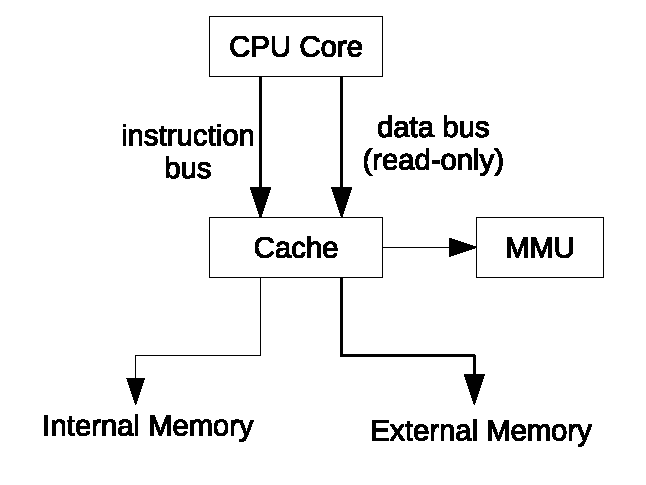
\includegraphics[width=0.5\textwidth]{./07-SYSMEM/figures/07-SYSMEM-cache-arch.eps}}
     \caption{Cache Structure}
    \label{fig:sysmem-cache-arch}
\end{figure}
 
\subsubsection{Cache Operations}

\chipname{} cache support the following operations:

\begin{enumerate}
\item \textbf{Invalidate}: This operation is used to clear valid data in the cache. After this operation is completed, the data will only be stored in the external memory. The CPU needs to access the external memory in order to read this data. There are two types of invalidate-operation: automatic invalidation (Auto-Invalidate) and manual invalidation (Manual-Invalidate). Manual-Invalidate is performed only on data in the specified area in the cache, while Auto-Invalidate is performed on all data in the cache.

\item \textbf{Preload}: This operation is used to load instructions and data into the cache in advance. The minimum unit of preload-operation is one block. There are two types of preload-operation: manual preload (Manual-Preload) and automatic preload (Auto-Preload). Manual-Preload means that the hardware prefetches a piece of continuous data according to the virtual address specified by the software. Auto-Preload means the hardware prefetches a piece of continuous data according to the current address where the cache hits or misses (depending on configuration).

\item \textbf{Lock/Unlock}: The lock operation is used to prevent the data in the cache from being easily replaced. There are two types of lock: prelock and manual lock. When prelock is enabled, the cache locks the data in the specified area when filling the missing data to cache memory, while the data outside the specified area will not be locked. When manual lock is enabled, the cache checks the data that is already in the cache memory and only locks the data in the specified area, and leaves the data outside the specified area unlocked. When there are missing data, the cache will replace the data in the unlocked way first, so the data in the locked way is always stored in the cache and will not be replaced. But when all ways within the cache are locked, the cache will replace data, as if it was not locked. Unlocking is the reverse of locking, except that it only can be done manually.

Please note that the Manual-Invalidate operations will only work on the unlocked data. If you expect to perform such operation on the locked data, please unlock them first.
\end{enumerate}



\subsection{GDMA Address Space}

The GDMA (General Direct Memory Access) peripheral in \chipname{} can provide DMA (Direct Memory Access) services including:

\begin{itemize}
    \item Data transfers between different locations of internal memory;
    \item Data transfers between modules/peripherals and internal memory.
\end{itemize}


GDMA uses the same addresses as the data bus to read and write Internal SRAM 1. Specifically, GDMA uses address range 0x3FC8\_0000 \verb+~+ 0x3FCD\_FFFF to access Internal SRAM 1. Note that GDMA cannot access the internal memory occupied by the cache.


There are \textcolor{red}{7} peripherals/modules that can work together with GDMA.

As shown in Figure \ref{fig:sysmem-gdma-peripheral},
these 7 vertical lines in turn correspond to these 7 peripherals/modules with GDMA function, the horizontal line represents a certain channel of GDMA (can be any channel), and the intersection of the vertical line and the horizontal line indicates that a peripheral/module has the ability to access the corresponding channel of GDMA. If there are multiple intersections on the same line, it means that these peripherals/modules cannot enable the GDMA function at the same time.



\begin{figure}[H]
    \centering
    \fbox{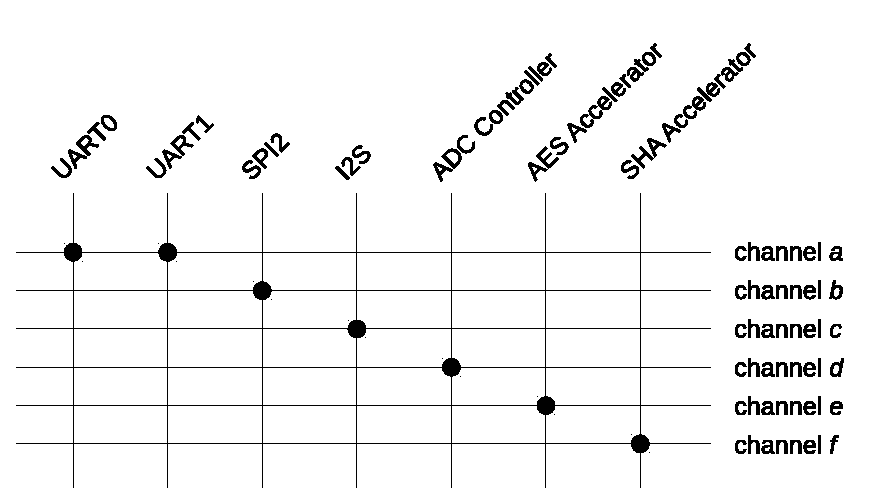
\includegraphics[width=0.9\textwidth]{./07-SYSMEM/figures/07-SYSMEM-GDMA-peripheral.eps}}
     \caption{Peripherals/modules that can work with GDMA}
    \label{fig:sysmem-gdma-peripheral}
\end{figure}
 

These peripherals/modules can access any memory available to GDMA. For more information, please refer to Chapter \ref{mod:dma} \textit{\nameref{mod:dma}}.

\begin{tiplisting}
\vspace{-2em}
\begin{enumerate}
    When accessing a memory via GDMA, a corresponding access permission is needed, otherwise this access may fail. For more information about permission control, please refer to Chapter \ref{mod:permctrl} \textit{\nameref{mod:permctrl}}.
\end{enumerate}
\end{tiplisting}


\subsection{Modules/Peripherals}

The CPU can access modules/peripherals via 0x6000\_0000 \verb+~+ 0x600D\_0FFF shared by the data/instruction bus.


\subsubsection{Module/Peripheral Address Mapping}

Table \ref{tab:sysmem-base-address} lists all the modules/peripherals and their respective address ranges. Note that the address space of specific modules/peripherals is defined by ``Boundary Address" (including both Low Address and High Address).

 \begin{longtable}[c]{ |p{5cm}|c|c|r|p{1.0cm}| } 
    
  \caption{Module/Peripheral Address Mapping}
  \label{tab:sysmem-base-address} 
\\\hline
  \rowcolor{lightgray}
       & \multicolumn{2}{c|}{\textbf{Boundary Address}} & & \\\cline{2-3}
       
       \rowcolor{lightgray}
       \multirow{-2}*{\textbf{Target}} & \textbf{Low Address} & \textbf{High Address} & \multirow{-2}*{\textbf{Size (KB)}} & \multirow{-2}*{\textbf{Notes}} \\\hline
    \endfirsthead
    
       \multicolumn{5}{c}{\bfseries \tablename\ \thetable{} -- cont'd from previous page}\\\hline
       
       \rowcolor{lightgray}
       & \multicolumn{2}{c|}{\textbf{Boundary Address}} & & \\\cline{2-3}
       
       \rowcolor{lightgray}
       \multirow{-2}*{\textbf{Target}} & \textbf{Low Address} & \textbf{High Address} & \multirow{-2}*{\textbf{Size (KB)}} & \multirow{-2}*{\textbf{Notes}} \\\hline
    \endhead
    
        \multicolumn{5}{r}{\textbf{Cont'd on next page}} \\
    \endfoot
    \endlastfoot
 
		                \hyperref[mod:uart]{UART Controller 0}           & 0x6000\_0000 & 0x6000\_0FFF &   4     &   \\\hline
    \rowcolor{gray!25}  Reserved                    & 0x6000\_1000 & 0x6000\_1FFF &         &   \\\hline
                        \hyperref[mod:spi]{SPI Controller 1}            & 0x6000\_2000 & 0x6000\_2FFF &   4     &   \\\hline
                        \hyperref[mod:spi]{SPI Controller 0}            & 0x6000\_3000 & 0x6000\_3FFF &   4     &   \\\hline
                        \hyperref[mod:iomuxgpio]{GPIO}                        & 0x6000\_4000 & 0x6000\_4FFF &   4     &   \\\hline
    \rowcolor{gray!25}  Reserved                    & 0x6000\_5000 & 0x6000\_6FFF &         &   \\\hline
    \rowcolor{gray!25}  Reserved  & 0x6000\_7000 & 0x6000\_7FFF &        &   \\\hline
                        \hyperref[mod:lowpowm]{Low-Power Management}        & 0x6000\_8000 & 0x6000\_8FFF &   4     &   \\\hline
                        \hyperref[mod:iomuxgpio]{IO MUX}                      & 0x6000\_9000 & 0x6000\_9FFF &   4     &   \\\hline
                
    \rowcolor{gray!25}  Reserved                    & 0x6000\_A000 & 0x6000\_FFFF &         &   \\\hline
                
                        \hyperref[mod:uart]{UART Controller 1}           & 0x6001\_0000 & 0x6001\_0FFF &   4     &   \\\hline
    \rowcolor{gray!25}  Reserved                    & 0x6001\_1000 & 0x6001\_2FFF &         &   \\\hline
                        \hyperref[mod:i2c]{I2C Controller}              & 0x6001\_3000 & 0x6001\_3FFF &   4     &   \\\hline
                        \hyperref[mod:uart]{UHCI0}                       & 0x6001\_4000 & 0x6001\_4FFF &   4     &   \\\hline
    \rowcolor{gray!25}  Reserved                    & 0x6001\_5000 & 0x6001\_5FFF &         &   \\\hline
                        \hyperref[mod:rmt]{Remote Control Peripheral}   & 0x6001\_6000 & 0x6001\_6FFF &   4     &   \\\hline
    \rowcolor{gray!25}  Reserved                    & 0x6001\_7000 & 0x6001\_8FFF &         &   \\\hline
                        \hyperref[mod:ledpwm]{LED PWM Controller}          & 0x6001\_9000 & 0x6001\_9FFF &   4     &   \\\hline
                        \hyperref[mod:efuse]{eFuse Controller}            & 0x6001\_A000 & 0x6001\_AFFF &   4     &   \\\hline
    \rowcolor{gray!25}  Reserved                    & 0x6001\_B000 & 0x6001\_EFFF &         &   \\\hline
                        \hyperref[mod:timg]{Timer Group 0}               & 0x6001\_F000 & 0x6001\_FFFF &   4     &   \\\hline
                        
                        \hyperref[mod:timg]{Timer Group 1}               & 0x6002\_0000 & 0x6002\_0FFF &   4     &   \\\hline
    \rowcolor{gray!25}  Reserved                    & 0x6002\_1000 & 0x6002\_2FFF &         &   \\\hline
                        \hyperref[mod:systimer]{System Timer}                & 0x6002\_3000 & 0x6002\_3FFF &   4     &   \\\hline
                        \hyperref[mod:spi]{SPI Controller 2}            & 0x6002\_4000 & 0x6002\_4FFF &   4     &   \\\hline
    \rowcolor{gray!25}  Reserved                    & 0x6002\_5000 & 0x6002\_5FFF &         &   \\\hline
                        \hyperref[mod:permctrl]{SYSCON}              & 0x6002\_6000 & 0x6002\_6FFF &   4     &   \\\hline
    \rowcolor{gray!25}  Reserved                    & 0x6002\_7000 & 0x6002\_AFFF &         &   \\\hline
                    \hyperref[mod:twai]{Two-wire Automotive Interface}   & 0x6002\_B000 & 0x6002\_BFFF &   4     &   \\\hline
    \rowcolor{gray!25}  Reserved                    & 0x6002\_C000 & 0x6002\_CFFF &         &   \\\hline
                        \hyperref[mod:i2s]{I2S Controller}              & 0x6002\_D000 & 0x6002\_DFFF &   4     &   \\\hline
    \rowcolor{gray!25}  Reserved                    & 0x6002\_E000 & 0x6003\_9FFF &         &   \\\hline

                        \hyperref[mod:aes]{AES Accelerator}             & 0x6003\_A000 & 0x6003\_AFFF &   4    &   \\\hline
                        \hyperref[mod:sha]{SHA Accelerator}             & 0x6003\_B000 & 0x6003\_BFFF &   4    &   \\\hline
                        \hyperref[mod:rsa]{RSA Accelerator}             & 0x6003\_C000 & 0x6003\_CFFF &   4    &   \\\hline
                        \hyperref[mod:digsig]{RSA Digital Signature Peripheral (RSA\_DS)}           & 0x6003\_D000 & 0x6003\_DFFF &   4    &   \\\hline
                        \hyperref[mod:hmac]{HMAC Accelerator}            & 0x6003\_E000 & 0x6003\_EFFF &   4    &   \\\hline
                        \hyperref[mod:dma]{GDMA Controller}             & 0x6003\_F000 & 0x6003\_FFFF &   4    &   \\\hline

                        \hyperref[mod:sensor]{ADC Controller}              & 0x6004\_0000 & 0x6004\_0FFF &   4    &   \\\hline
    \rowcolor{gray!25}  Reserved                    & 0x6004\_1000 & 0x6002\_FFFF &        &   \\\hline
                        \hyperref[mod:usbserialjtag]{USB Serial/JTAG Controller}  & 0x6004\_3000 & 0x6004\_3FFF &   4    &  \\\hline
    \rowcolor{gray!25}  Reserved                    & 0x6004\_4000 & 0x600B\_FFFF &        &   \\\hline
                        
                        \hyperref[mod:sysreg]{System Registers}            & 0x600C\_0000 & 0x600C\_0FFF &   4    &   \\\hline
                        \hyperref[mod:permctrl]{PMS Registers }         & 0x600C\_1000 & 0x600C\_1FFF &   4    &   \\\hline 
                        \hyperref[mod:intmtrx]{Interrupt Matrix}            & 0x600C\_2000 & 0x600C\_2FFF &   4    &   \\\hline
    \rowcolor{gray!25}  Reserved                    & 0x600C\_3000 & 0x600C\_3FFF &        &   \\\hline
    \rowcolor{gray!25}  Reserved              & 0x600C\_4000 & 0x600C\_BFFF &      &   \\\hline
        \hyperref[mod:extmemencr]{External Memory Encryption and Decryption}   & 0x600C\_C000 & 0x600C\_CFFF &   4    &   \\\hline
    \rowcolor{gray!25}  Reserved                    & 0x600C\_D000 & 0x600C\_DFFF &        &   \\\hline
                        \hyperref[mod:dbgassist]{Assist Debug}                & 0x600C\_E000 & 0x600C\_EFFF &   4    &   \\\hline
    \rowcolor{gray!25}  Reserved                    & 0x600C\_F000 & 0x600C\_FFFF &        &   \\\hline
                        \hyperref[mod:wctrl]{World Controller}            & 0x600D\_0000 & 0x600D\_0FFF &   4    &   \\\hline
    
\end{longtable}







\end{document}
